\documentclass[12pt,a4paper]{article}
\usepackage{lmodern}
\usepackage{amssymb,amsmath}
\usepackage{ifxetex,ifluatex}
\usepackage{fixltx2e} % provides \textsubscript
\ifnum 0\ifxetex 1\fi\ifluatex 1\fi=0 % if pdftex
  \usepackage[T1]{fontenc}
  \usepackage[utf8]{inputenc}
\else % if luatex or xelatex
  \ifxetex
    \usepackage{mathspec}
  \else
    \usepackage{fontspec}
  \fi
  \defaultfontfeatures{Ligatures=TeX,Scale=MatchLowercase}
\fi
% use upquote if available, for straight quotes in verbatim environments
\IfFileExists{upquote.sty}{\usepackage{upquote}}{}
% use microtype if available
\IfFileExists{microtype.sty}{%
\usepackage{microtype}
\UseMicrotypeSet[protrusion]{basicmath} % disable protrusion for tt fonts
}{}
\usepackage[margin=2cm]{geometry}
\usepackage{hyperref}
\hypersetup{unicode=true,
            pdftitle={Content Analysis of Scaling Up Nutrition (SUN) Movement Progress Reports from 2011-2017},
            pdfauthor={Ernest Guevarra},
            pdfborder={0 0 0},
            breaklinks=true}
\urlstyle{same}  % don't use monospace font for urls
\usepackage{color}
\usepackage{fancyvrb}
\newcommand{\VerbBar}{|}
\newcommand{\VERB}{\Verb[commandchars=\\\{\}]}
\DefineVerbatimEnvironment{Highlighting}{Verbatim}{commandchars=\\\{\}}
% Add ',fontsize=\small' for more characters per line
\usepackage{framed}
\definecolor{shadecolor}{RGB}{248,248,248}
\newenvironment{Shaded}{\begin{snugshade}}{\end{snugshade}}
\newcommand{\KeywordTok}[1]{\textcolor[rgb]{0.13,0.29,0.53}{\textbf{#1}}}
\newcommand{\DataTypeTok}[1]{\textcolor[rgb]{0.13,0.29,0.53}{#1}}
\newcommand{\DecValTok}[1]{\textcolor[rgb]{0.00,0.00,0.81}{#1}}
\newcommand{\BaseNTok}[1]{\textcolor[rgb]{0.00,0.00,0.81}{#1}}
\newcommand{\FloatTok}[1]{\textcolor[rgb]{0.00,0.00,0.81}{#1}}
\newcommand{\ConstantTok}[1]{\textcolor[rgb]{0.00,0.00,0.00}{#1}}
\newcommand{\CharTok}[1]{\textcolor[rgb]{0.31,0.60,0.02}{#1}}
\newcommand{\SpecialCharTok}[1]{\textcolor[rgb]{0.00,0.00,0.00}{#1}}
\newcommand{\StringTok}[1]{\textcolor[rgb]{0.31,0.60,0.02}{#1}}
\newcommand{\VerbatimStringTok}[1]{\textcolor[rgb]{0.31,0.60,0.02}{#1}}
\newcommand{\SpecialStringTok}[1]{\textcolor[rgb]{0.31,0.60,0.02}{#1}}
\newcommand{\ImportTok}[1]{#1}
\newcommand{\CommentTok}[1]{\textcolor[rgb]{0.56,0.35,0.01}{\textit{#1}}}
\newcommand{\DocumentationTok}[1]{\textcolor[rgb]{0.56,0.35,0.01}{\textbf{\textit{#1}}}}
\newcommand{\AnnotationTok}[1]{\textcolor[rgb]{0.56,0.35,0.01}{\textbf{\textit{#1}}}}
\newcommand{\CommentVarTok}[1]{\textcolor[rgb]{0.56,0.35,0.01}{\textbf{\textit{#1}}}}
\newcommand{\OtherTok}[1]{\textcolor[rgb]{0.56,0.35,0.01}{#1}}
\newcommand{\FunctionTok}[1]{\textcolor[rgb]{0.00,0.00,0.00}{#1}}
\newcommand{\VariableTok}[1]{\textcolor[rgb]{0.00,0.00,0.00}{#1}}
\newcommand{\ControlFlowTok}[1]{\textcolor[rgb]{0.13,0.29,0.53}{\textbf{#1}}}
\newcommand{\OperatorTok}[1]{\textcolor[rgb]{0.81,0.36,0.00}{\textbf{#1}}}
\newcommand{\BuiltInTok}[1]{#1}
\newcommand{\ExtensionTok}[1]{#1}
\newcommand{\PreprocessorTok}[1]{\textcolor[rgb]{0.56,0.35,0.01}{\textit{#1}}}
\newcommand{\AttributeTok}[1]{\textcolor[rgb]{0.77,0.63,0.00}{#1}}
\newcommand{\RegionMarkerTok}[1]{#1}
\newcommand{\InformationTok}[1]{\textcolor[rgb]{0.56,0.35,0.01}{\textbf{\textit{#1}}}}
\newcommand{\WarningTok}[1]{\textcolor[rgb]{0.56,0.35,0.01}{\textbf{\textit{#1}}}}
\newcommand{\AlertTok}[1]{\textcolor[rgb]{0.94,0.16,0.16}{#1}}
\newcommand{\ErrorTok}[1]{\textcolor[rgb]{0.64,0.00,0.00}{\textbf{#1}}}
\newcommand{\NormalTok}[1]{#1}
\usepackage{graphicx,grffile}
\makeatletter
\def\maxwidth{\ifdim\Gin@nat@width>\linewidth\linewidth\else\Gin@nat@width\fi}
\def\maxheight{\ifdim\Gin@nat@height>\textheight\textheight\else\Gin@nat@height\fi}
\makeatother
% Scale images if necessary, so that they will not overflow the page
% margins by default, and it is still possible to overwrite the defaults
% using explicit options in \includegraphics[width, height, ...]{}
\setkeys{Gin}{width=\maxwidth,height=\maxheight,keepaspectratio}
\IfFileExists{parskip.sty}{%
\usepackage{parskip}
}{% else
\setlength{\parindent}{0pt}
\setlength{\parskip}{6pt plus 2pt minus 1pt}
}
\setlength{\emergencystretch}{3em}  % prevent overfull lines
\providecommand{\tightlist}{%
  \setlength{\itemsep}{0pt}\setlength{\parskip}{0pt}}
\setcounter{secnumdepth}{0}
% Redefines (sub)paragraphs to behave more like sections
\ifx\paragraph\undefined\else
\let\oldparagraph\paragraph
\renewcommand{\paragraph}[1]{\oldparagraph{#1}\mbox{}}
\fi
\ifx\subparagraph\undefined\else
\let\oldsubparagraph\subparagraph
\renewcommand{\subparagraph}[1]{\oldsubparagraph{#1}\mbox{}}
\fi

%%% Use protect on footnotes to avoid problems with footnotes in titles
\let\rmarkdownfootnote\footnote%
\def\footnote{\protect\rmarkdownfootnote}

%%% Change title format to be more compact
\usepackage{titling}

% Create subtitle command for use in maketitle
\newcommand{\subtitle}[1]{
  \posttitle{
    \begin{center}\large#1\end{center}
    }
}

\setlength{\droptitle}{-2em}
  \title{Content Analysis of Scaling Up Nutrition (SUN) Movement Progress Reports
from 2011-2017}
  \pretitle{\vspace{\droptitle}\centering\huge}
  \posttitle{\par}
  \author{Ernest Guevarra}
  \preauthor{\centering\large\emph}
  \postauthor{\par}
  \predate{\centering\large\emph}
  \postdate{\par}
  \date{17/05/2018}


\begin{document}
\maketitle

\hypertarget{re-structure-dataset-into-a-one-token-per-row-format}{%
\subsection{Re-structure dataset into a one-token-per-row
format}\label{re-structure-dataset-into-a-one-token-per-row-format}}

\begin{Shaded}
\begin{Highlighting}[]
\NormalTok{tidy_reports <-}\StringTok{ }\KeywordTok{progress_reports}\NormalTok{() }\OperatorTok
\StringTok{  }\KeywordTok{unnest_tokens}\NormalTok{(word, text)}
  
\NormalTok{tidy_reports}
\end{Highlighting}
\end{Shaded}

\begin{verbatim}
## # A tibble: 354,209 x 5
##     page linenumber chapter  year word   
##    <int>      <int>   <int> <int> <chr>  
##  1     3          1       0  2011 preface
##  2     3          2       0  2011 one    
##  3     3          2       0  2011 year   
##  4     3          2       0  2011 ago    
##  5     3          2       0  2011 i      
##  6     3          2       0  2011 joined 
##  7     3          2       0  2011 a      
##  8     3          2       0  2011 group  
##  9     3          2       0  2011 of     
## 10     3          2       0  2011 leaders
## # ... with 354,199 more rows
\end{verbatim}

\hypertarget{remove-stop-words---words-not-useful-in-analysis}{%
\subsection{Remove stop words - words not useful in
analysis}\label{remove-stop-words---words-not-useful-in-analysis}}

\begin{Shaded}
\begin{Highlighting}[]
\KeywordTok{data}\NormalTok{(stop_words)}

\NormalTok{tidy_reports <-}\StringTok{ }\NormalTok{tidy_reports }\OperatorTok
\StringTok{  }\KeywordTok{anti_join}\NormalTok{(stop_words)}
\end{Highlighting}
\end{Shaded}

\begin{verbatim}
## Joining, by = "word"
\end{verbatim}

\hypertarget{find-the-most-common-words-in-all-the-reports-as-a-whole}{%
\subsection{Find the most common words in all the reports as a
whole}\label{find-the-most-common-words-in-all-the-reports-as-a-whole}}

\begin{Shaded}
\begin{Highlighting}[]
\NormalTok{tidy_reports }\OperatorTok
\StringTok{  }\KeywordTok{count}\NormalTok{(word, }\DataTypeTok{sort =} \OtherTok{TRUE}\NormalTok{)}
\end{Highlighting}
\end{Shaded}

\begin{verbatim}
## # A tibble: 12,659 x 2
##    word          n
##    <chr>     <int>
##  1 nutrition  5932
##  2 sun        3050
##  3 countries  2302
##  4 national   1914
##  5 movement   1843
##  6 country    1552
##  7 2015       1377
##  8 progress   1308
##  9 2016       1199
## 10 2014       1174
## # ... with 12,649 more rows
\end{verbatim}

\hypertarget{visualise-the-most-common-words}{%
\subsection{Visualise the most common
words}\label{visualise-the-most-common-words}}

\begin{Shaded}
\begin{Highlighting}[]
\NormalTok{tidy_reports }\OperatorTok
\StringTok{  }\KeywordTok{count}\NormalTok{(word, }\DataTypeTok{sort =} \OtherTok{TRUE}\NormalTok{) }\OperatorTok
\StringTok{  }\KeywordTok{filter}\NormalTok{(n }\OperatorTok{>}\StringTok{ }\DecValTok{600}\NormalTok{) }\OperatorTok
\StringTok{  }\KeywordTok{mutate}\NormalTok{(}\DataTypeTok{word =} \KeywordTok{reorder}\NormalTok{(word, n)) }\OperatorTok
\StringTok{  }\KeywordTok{ggplot}\NormalTok{(}\KeywordTok{aes}\NormalTok{(word, n)) }\OperatorTok{+}\StringTok{ }
\StringTok{  }\KeywordTok{geom_col}\NormalTok{() }\OperatorTok{+}\StringTok{ }
\StringTok{  }\KeywordTok{xlab}\NormalTok{(}\OtherTok{NULL}\NormalTok{) }\OperatorTok{+}\StringTok{ }
\StringTok{  }\KeywordTok{coord_flip}\NormalTok{()}
\end{Highlighting}
\end{Shaded}

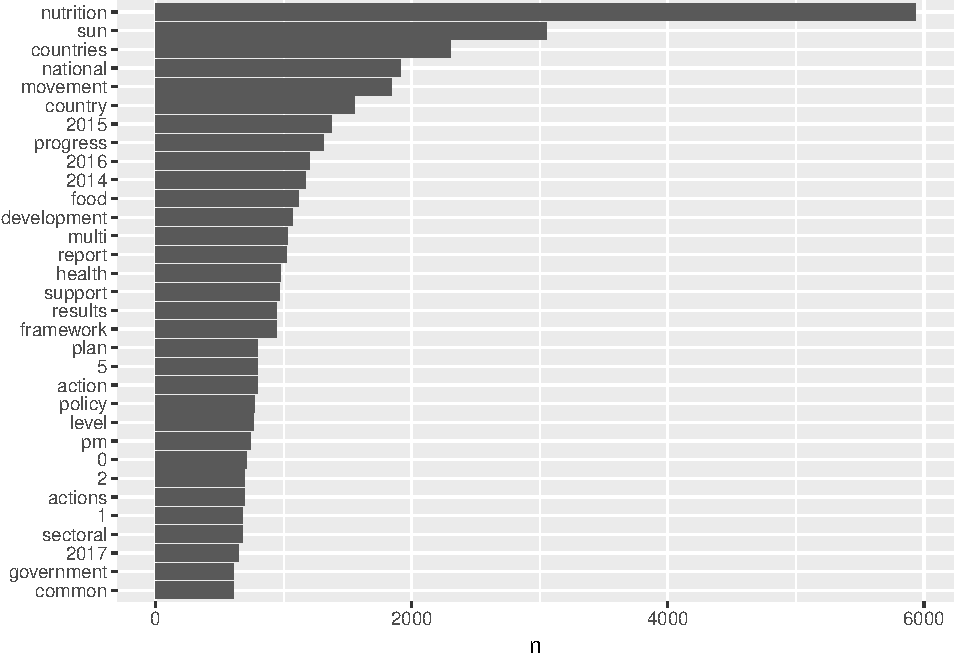
\includegraphics{progressSUN_files/figure-latex/unnamed-chunk-4-1.pdf}

\begin{Shaded}
\begin{Highlighting}[]
\NormalTok{nrc_joy <-}\StringTok{ }\KeywordTok{get_sentiments}\NormalTok{(}\StringTok{"nrc"}\NormalTok{) }\OperatorTok\StringTok{ }
\StringTok{  }\KeywordTok{filter}\NormalTok{(sentiment }\OperatorTok{==}\StringTok{ "joy"}\NormalTok{)}

\NormalTok{tidy_reports }\OperatorTok
\StringTok{  }\KeywordTok{filter}\NormalTok{(year }\OperatorTok{==}\StringTok{ }\DecValTok{2011}\NormalTok{) }\OperatorTok
\StringTok{  }\KeywordTok{inner_join}\NormalTok{(nrc_joy) }\OperatorTok
\StringTok{  }\KeywordTok{count}\NormalTok{(word, }\DataTypeTok{sort =} \OtherTok{TRUE}\NormalTok{)}
\end{Highlighting}
\end{Shaded}

\begin{verbatim}
## Joining, by = "word"
\end{verbatim}

\begin{verbatim}
## # A tibble: 62 x 2
##    word            n
##    <chr>       <int>
##  1 sun           236
##  2 food          105
##  3 progress       72
##  4 child          35
##  5 resources      30
##  6 weight         19
##  7 birth          18
##  8 improve        17
##  9 established    15
## 10 engaged        13
## # ... with 52 more rows
\end{verbatim}

\begin{Shaded}
\begin{Highlighting}[]
\NormalTok{progress_sentiment <-}\StringTok{ }\NormalTok{tidy_reports }\OperatorTok
\StringTok{  }\KeywordTok{inner_join}\NormalTok{(}\KeywordTok{get_sentiments}\NormalTok{(}\StringTok{"bing"}\NormalTok{)) }\OperatorTok
\StringTok{  }\KeywordTok{count}\NormalTok{(year, }\DataTypeTok{index =}\NormalTok{ linenumber }\OperatorTok\StringTok{ }\DecValTok{80}\NormalTok{, sentiment) }\OperatorTok
\StringTok{  }\KeywordTok{spread}\NormalTok{(sentiment, n, }\DataTypeTok{fill =} \DecValTok{0}\NormalTok{) }\OperatorTok
\StringTok{  }\KeywordTok{mutate}\NormalTok{(}\DataTypeTok{sentiment =}\NormalTok{ positive }\OperatorTok{-}\StringTok{ }\NormalTok{negative)}
\end{Highlighting}
\end{Shaded}

\begin{verbatim}
## Joining, by = "word"
\end{verbatim}

\begin{Shaded}
\begin{Highlighting}[]
\KeywordTok{ggplot}\NormalTok{(progress_sentiment, }\KeywordTok{aes}\NormalTok{(index, sentiment, }\DataTypeTok{fill =}\NormalTok{ year)) }\OperatorTok{+}
\StringTok{  }\KeywordTok{geom_col}\NormalTok{(}\DataTypeTok{show.legend =} \OtherTok{FALSE}\NormalTok{) }\OperatorTok{+}
\StringTok{  }\KeywordTok{facet_wrap}\NormalTok{(}\OperatorTok{~}\NormalTok{year, }\DataTypeTok{ncol =} \DecValTok{2}\NormalTok{, }\DataTypeTok{scales =} \StringTok{"free_x"}\NormalTok{)}
\end{Highlighting}
\end{Shaded}

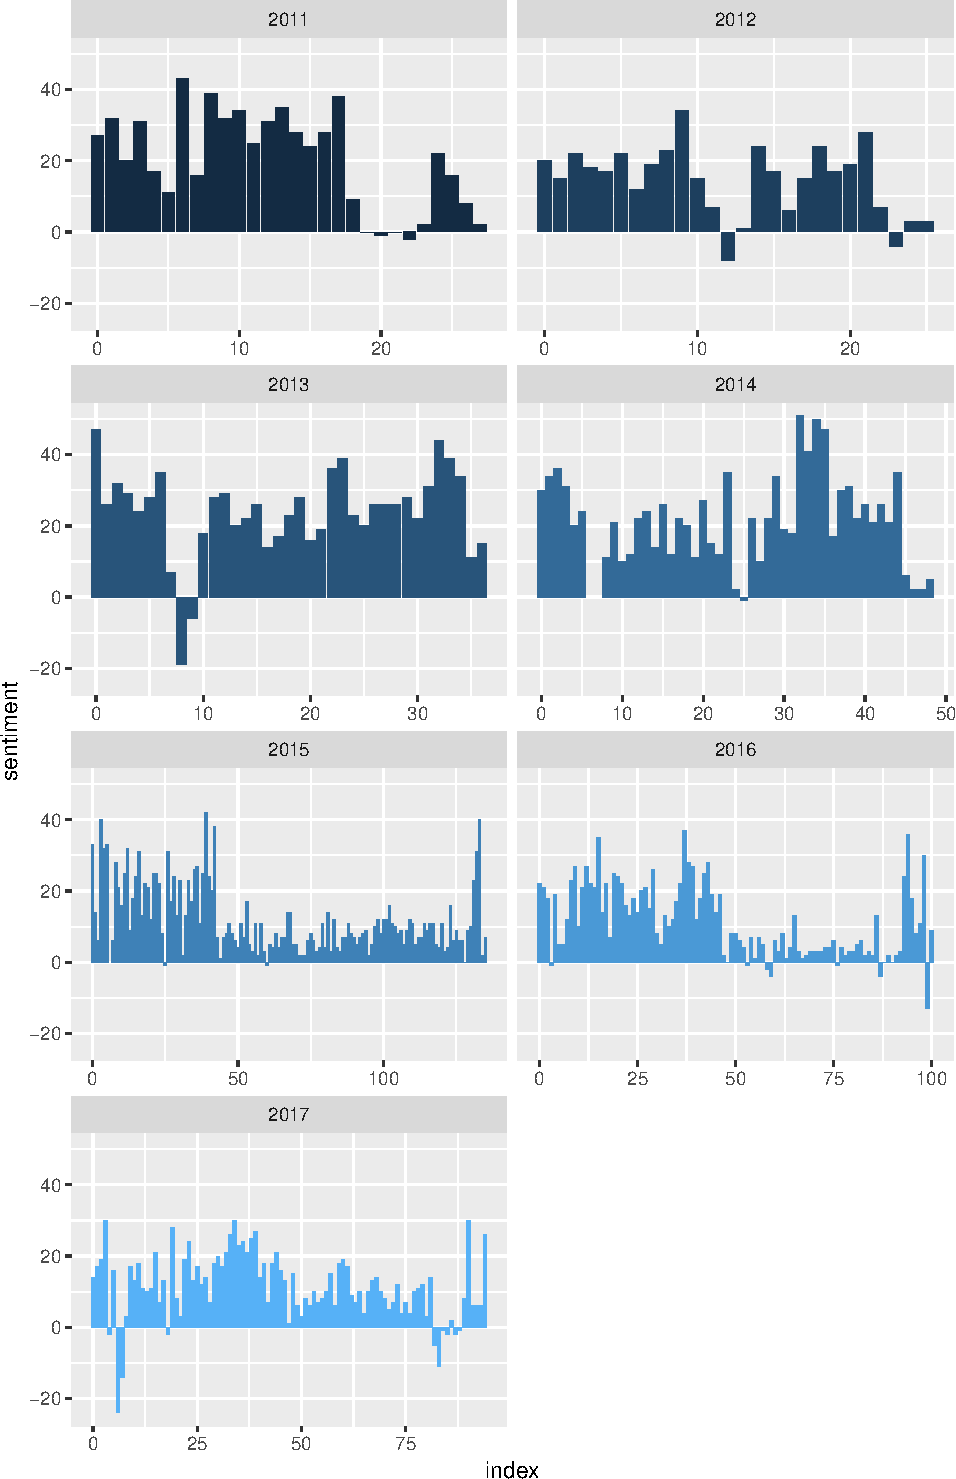
\includegraphics{progressSUN_files/figure-latex/unnamed-chunk-7-1.pdf}


\end{document}
